\documentclass{sigplanconf}
\usepackage{version}
\usepackage{graphicx}
\usepackage{amsmath}
\usepackage{mathptmx}
\usepackage{style/utils}
\usepackage{style/code}
\usepackage{url}


% -----------------------------------------------------------------------------
\begin{document}
\title	{Guiding Parallel Array Fusion with Indexed Types}

\authorinfo{ 
  Ben Lippmeier$^\dagger$
  \and Manuel M. T. Chakravarty$^\dagger$
  \and Gabriele Keller$^\dagger$
  \and Simon Peyton Jones$^\ddagger$

}{
  \vspace{5pt}
  \shortstack{
    $^\dagger$Computer Science and Engineering \\
    University of New South Wales, Australia \\[2pt]
    \textsf{\{benl,chak,keller\}@cse.unsw.edu.au}
  }
  \and
  \shortstack{
    $^\ddagger$Microsoft Research Ltd \\
    Cambridge, England \\[2pt]
    \textsf{\{simonpj\}@microsoft.com}
  }
}

\conferenceinfo{Haskell'12,} {September 13, 2012, Copenhagen, Denmark.}
\CopyrightYear{2012}
\copyrightdata{978-1-4503-1574-6/12/09}

\maketitle
\makeatactive


% -----------------------------------------------------------------------------
\begin{abstract}
We present a refined approach to parallel array fusion that uses indexed types to specify the internal representation of each array. Our approach aids the client programmer in reasoning about the performance of their program in terms of the source code. It also makes the intermediate code easier to transform at compile-time, resulting in faster compilation and more reliable runtimes. We demonstrate how our new approach improves both the clarity and performance of several end-user written programs, including a fluid flow solver and an interpolator for volumetric data.
\end{abstract}

\category
	{D.3.3}
	{Programming Languages}
	{Language Constructs and Features---Concurrent programming structures; Polymorphism; Abstract data types}

\terms
	Languages, Performance

\keywords
	Arrays, Data parallelism, Haskell


% -----------------------------------------------------------------------------
%!TEX root = ../Main.tex
\section{Introdution}

The Haskell library ecosystem is blessed with a multitude of libraries for writing streaming data flow programs. Stand out examples include iteratee CITE, enumerator CITE, conduit CITE and pipes CITE. These libraries are based around ... and more recent examples such as pipes provide a useful set of algebraic equivalences that give a clean mathematical structure to the provided mathemetical structure.

Libraries such as iteratee and enumerator are typically used to deal with data sets that do not fit in main memory, as the constant space guarantee ensures that the program will run to completion without suffering an out-of-memory error. However, current computing platforms use multi-core processors, the programming models provided by such streaming libraries do not also provide a notion of \emph{parallelism} to help deal with the implied amount of data. They also lack support for branching data flows where produced streams can be consumed by several consumers without the programmer needing to had fuse them.

We provide several techniques that increase the scope of programs that can be written in such libraries. Our target applications concern \emph{medium data}, meaning data that is large enough that it does not fit in the main memory of a normal desktop machine, but not so large that we require a cluster of multiple physical machines. For a lesser amount of data one could simply load the data into main memory and use an in-memory array library such as CITE or CITE. For greater data one needs to turn to a distributed system such as Hadoop or Spark and deal with the unreliable network and lack of shared memory. Repa Flow targets the sweet middle ground.

We make the following contributions:

\begin{itemize}
\item Our parallel data flows consist of a bundle of streams, where each stream can process a separate partition of a data set on a separate processor core.

\item Our API uses polarised flow endpoints (@Sources@ and @Sinks@) to ensure that programs run in constant space. We demonstrate how this standard technique can be extended to branching data flows, where produced flows are consumed by multiple consumers.

\item The data processed by our streams is chunked so that each operation processes several elements at a time. We show how to design the core API in a generic fashion so that chunk-at-a-time operators can interoperate smoothly with element-at-a-time operators.
\TODO{We don't support leftovers}

\item We show how to use Continuation Passing Style to provoke the Glasgow Haskell Compiler into applying stream fusion across chunks processed by independent flow operators. For example, the map-map fusion on flows arises naturally from map-map fusion rule on chunks (arrays) of elements.
\end{itemize}

Our work is embodied in Repa Flow, which is available on Hackage. \TODO{Specify the relationship to previous work on Repa}. This is a new layer on the original delayed arrays of our original Repa library.



\section{Representation, Fusion, and Code Explosion}
\label{section:problem}

\begin{figure}
\begin{small}
\begin{code}
data Array sh e = Manifest sh (Vector e)
                | Delayed  sh (sh -> e)

class Shape sh where
   toIndex      :: sh -> sh -> Int
   fromIndex    :: sh -> Int -> sh
   size         :: sh -> Int
   ...more operations...
data DIM1 = DIM1 !Int
data DIM2 = DIM2 !Int !Int
...more dimensions...

index :: Shape sh => Array sh e -> sh -> e
index (Delayed sh f)    ix = f ix
index (Manifest sh vec) ix = indexV vec (toIndex sh ix)

delay :: Shape sh => Array sh e -> (sh, sh -> e)
delay (Delayed  sh f)   = (sh, f)
delay (Manifest sh vec) 
 = (sh, \ix -> indexV vec (toIndex sh ix))

map :: Shape sh => (a -> b) -> Array sh a -> Array sh b
map f arr = let (sh, g) = delay arr 
            in  Delayed sh (f . g)

zipWith :: Shape sh => (a -> b -> c) 
        -> Array sh a -> Array sh b -> Array sh c
zipWith f arr1 arr2
 = let  (sh1,  f1)       = delay arr1
        (_sh2, f2)       = delay arr2
        get ix          = f (f1 ix) (f2 ix)
   in   Delayed sh1 get

force :: Shape sh => Array sh e -> Array sh e
force arr 
 = unsafePerformIO
 $ case arr of
    Manifest sh vec    
     ->     return  $ Manifest sh vec
    Delayed sh f    
     -> do  mvec    <- unsafeNew (size sh)
            fill (size sh) mvec (f . fromIndex sh)
            vec     <- unsafeFreeze mvec
            return  $ Manifest sh vec
\end{code}
\caption{Essential Repa Version 1 Definitions}
\label{figure:Repa1}
\end{small}
\end{figure}

We start by reviewing the design problems of original Repa library. A simplified version of the core definitions of Repa~1~\cite{Keller:Repa} is in Figure~\ref{figure:Repa1}. Repa~2 extends the @Array@ type to support more efficient convolutions~\cite{Lippmeier:Stencil}, which we discuss in \S\ref{section:Explosion}.

Repa~1 introduced \emph{delayed arrays} to fuse multiple array operations, and minimise the overhead of \emph{index-space transforms}. Delayed arrays are represented by a function from indices to array elements, as we see in the definition of @Array@ Figure~\ref{figure:Repa1}. Delayed arrays contrast with \emph{manifest} arrays, which are represented as contiguous blocks of unboxed values. Fusion of operations on delayed arrays amounts to function composition, as we see in the definition of @map@. This gives us the map/map fusion rule, @map f . map g = map (f . g)@, for free and works similarly for many other operations, including index space transforms such as permutation, replication, slicing, and so on.

The elements of a multi-dimensional @Manifest@ array are stored in row-major order in a flat, one-dimensional @Vector@. The @Shape@ class holds operations to convert between higher-dimensional index types, such as @DIM2@, and the flat representation. In particular, the @toIndex@ and @fromIndex@ functions convert between higher-dimensional and linear indices, and @size@ yields the total number of elements in an array of the given shape. Based on the methods of the @Shape@ class, the function @index@ retrieves a single element from an array, and @delay@ produces an array's shape together with an indexing function to move to the delayed representation. (The function @indexV@ indexes into the flat @Vector@.)

As stated in the introduction, although Repa 1 \& 2 can produce efficient code on both sequential and parallel machines~\cite{Keller:Repa,Lippmeier:Stencil}, they have some significant shortcomings, which we review next.


% -----------------------------------------------------------------------------
\subsection{Problem 1: Not Applying {\texttt force}}
\label{section:force}

To illustrate the problems with Repa 1, we will reuse the example from the introduction:
%
\begin{small}
\begin{code}
    doubleZip :: Array DIM2 Int -> Array DIM2 Int 
              -> Array DIM2 Int
    doubleZip arr1 arr2
     = map (* 2) $ zipWith (+) arr1 arr2
\end{code}
\end{small}

\eject
By inlining the definitions from Figure~\ref{figure:Repa1} and simplifying, we see that the composition of @map@ and @zipWith@ fuses to produce the following:
%
\begin{small}
\begin{code}
    let (sh1,  f1) = delay arr1
        (_sh2, f2) = delay arr2
        get ix     = (f1 ix + f2 ix) * 2
    in Delayed sh1 get
\end{code}
\end{small}
%
The problem is that the array returned by @map@ is not a \emph{manifest} array, so is not represented as real unboxed data in a contiguous block of memory. Instead, it is a \emph{delayed} array, represented by a function that takes an array index and computes each element on the fly. The fused code immediately builds a new @Delayed@ array without doing any actual work. This is problematic if the consumer of a delayed array uses elements multiple times. The elements will be recomputed each time, so sharing of results is lost along with runtime performance.

If we desire an array represented by real data, then we should use Repa's @force@ function, which turns a delayed array into a manifest array by executing loop-based parallel array filling code. We would use it in @doubleZip@ as follows:
%
\begin{small}
\begin{code}
    doubleZip arr1 arr2
     = force $ map (* 2) $ zipWith (+) arr1 arr2
\end{code}
\end{small}
%
The code here fuses @map@ and @zipWith@ by building a new Delayed array as before. It then fills a freshly-allocated @Manifest@ array, \emph{in parallel}, using the element-generating function stored in the new @Delayed@ array. In other words, the compiled code will contain an unfolding of the imperative loop provided by @force@, where the body performs the per-element function, here @(f1 ix + f2 ix) * 2@, where @f1@ and @f2@ retrieve elements from the two input arrays. 

Although our entire approach to parallel array programming hinges on the correct use of @force@, the type presented in the Repa~1 API documentation was rather uninformative:

\begin{small}
\begin{code}
  force :: Shape sh => Array sh a -> Array sh a
  -- Force an array, so that it becomes Manifest.
\end{code}
\end{small}
%
From its type alone, @force@ looks like an instance of the identity function. This coupled with the rather cryptic comment, led many users to overlook @force@ entirely. Poor documentation aside, our foundational view that ``a type is a name for a set of values'' was of no help in expressing the fact that ``if you don't use this function your program will be really slow''. 


% -----------------------------------------------------------------------------
\subsection{Problem 2: Runtime Representation Tests}
\label{section:rep-tests}

The version of @doubleZip@ using @force@ produces fused, loop-based code, but is still slower than a straightforward imperative version. This is because the @Array@ type has two data constructors, @Delayed@ and @Manifest@, so indexing functions must perform a run-time test to distinguish between them. This is a catastrophe if the test is in an inner loop, which is the native environment for indexing functions. In some cases GHC can lift such tests out of loops, but in general such transformations are unsound, because they can change strictness properties if the loop can perform no iterations.

Tantalisingly, the representation of an array at a particular program point does not change from run to run. The programmer always knows which representation is expected --- but, in Repa 1 \& 2 they lack a convenient way to express that knowledge. For example, if we know that only manifest arrays will be passed to @doubleZip@, then we should reify this fact by using explicit pattern matching:
\par
\begin{small}
\begin{code}
  doubleZip arr1@Manifest{} arr2@Manifest{}
   = force $ map (* 2) $ zipWith (+) arr1 arr2
\end{code}
\end{small}
%
While this version runs fast, it is awkward due to the implicit precondition: we need to ensure that all callers of @doubleZip@ force the arguments to ensure that they are manifest. 

The test for array representation is not the only run-time test that tends to be needlessly performed in an inner loop. An array also contains size information such as its width and height, which is often used in each iteration. As these are boxed @Int@ values, a loop might repeatedly unbox them, wasting cycles. To ensure the values are unboxed only once, in the preamble of the loop, we need to place a demand on them at the function entry point. We typically do this using bang patterns in the pattern that matches @Manifest@, and it turns out we also want to demand the flat vector to ensure its components are unboxed as well:
%
\begin{small}
\begin{code}
  doubleZip arr1@(Manifest !_ !_) arr2@(Manifest !_ !_)
  = force $ map (* 2) $ zipWith (+) arr1 arr2
\end{code}
\end{small}
%
Finally, @doubleZip@ runs as fast as a hand-written imperative loop. Unfortunately, the optimisations require reasoning that is not obvious from the source program, demand a deeper understanding of the compilation method than most users will have, and add a precondition that is not captured in the function signature.


% -----------------------------------------------------------------------------
\subsection{Problem 3: Inlining and Code Explosion}
\label{section:Explosion}

In a FORTRAN or C program, the programmer writes explicit loops. In Repa, the programmer never writes loops; the loops are in library functions. With respect to Figure~\ref{figure:Repa1}, the key loop is in the definition of @fill@, which is called by @force@. The loop code itself is too big to include here, but see \cite{Lippmeier:Stencil} for a full definition. The array operations such as @map@, @zipWith@ and so on, build @Delayed@ arrays by composing functions, but do not contain loops.

How does this turn into efficient code? Consider the last, most efficient version of @doubleZip@. Inlining @zipWith@, @map@, @delay@, and @force@, then simplifying yields:
\par
\begin{small}
\begin{code}
  doubleZip (Manifest !sh1 !vec1) (Manifest !_sh2 !vec2) 
   = unsafePerformIO 
   $ do mvec <- unsafeNew (size sh1) 
        fill (size sh1) mvec
          (\ix -> (indexV vec1 ix + indexV vec2 ix) * 2)
        vec <- unsafeFreeze mvec
        return $ Manifest sh1 vec
\end{code}
\end{small}
%
The pattern matching in @zipWith@'s calls to @delay@ are cancelled by the explicitly @Manifest@ arrays; the @Delayed@ array produced by @zipWith@ is canceled by the pattern match in @map@'s use of @delay@; and so on. When the definition of @fill@ is inlined, we get a tight loop, in which the output is built directly from the input vectors (@vec1@, @vec2@) without any intermediates.

Clearly, this fusion depends critically on (a) aggressive inlining and (b) cancellation of statically-visible array construction and pattern matching.  However, for efficient stencil convolution, we developed a more complex array representation~\cite{Lippmeier:Stencil}, similar to this:
\par
\begin{small}
\begin{code}
  data Array sh a 
    = Array { arrayExtent  :: sh
            , arrayRegions :: [Region sh a] }
\end{code}
\end{small}
%
Rather than just being @Manifest@ or @Delayed@, these arrays consist of a list of rectangular \emph{regions}. Each region has its own element-generating function, which is used to speed up the handling of boundary conditions.

Alas, this representation is fatal for the inline-and-cancel story outlined above. This is because the list @arrayRegions@ must be processed by a \emph{recursive} function, and compilers (including GHC) are rightly cautious about unrolling recursive functions. In a typical application the programmer knows the exact number of regions at any program point, say four boundaries and a central region. Unrolling five times here would be perfect, but the compiler does not know this.

\eject
To make this work, we ended up manually unrolling code in the library functions, by pattern matching on the region list. Here is a typical chunk of Repa 2 library code:
\par
\begin{small}
\begin{code}
  forceWith2 :: (Int -> a -> IO ())
             -> Array DIM2 a -> IO ()
  forceWith2 write arr
   = case arr of
      Array sh [r1]
       -> do fillRegion2P write sh r1
      Array sh [r1, r2]
       -> do fillRegion2P write sh r1
             fillRegion2P write sh r2
      Array sh [r1, r2, r3]
       -> do fillRegion2P write sh r1
             fillRegion2P write sh r2
             fillRegion2P write sh r3
      ...
      Array sh regions
       ->    mapM_ (fillRegion2P write sh) regions
\end{code}
\end{small}       
%
The details are not important, but it should be clear from the form how gruesome this is:
\begin{itemize}
\item The library only efficiently accommodates a maximum number of regions. If we use the final alternative of @forceWith2@ above, then the code will not fuse.
\item There is much repetition in the library code.
\item The library functions become very large because of the duplication, but they must still be inlined!
\end{itemize}
%
Aggressive use of @INLINE@ pragmas produces enormous intermediate programs, which we hope will then shrink radically through construction/pattern-matching cancellation. Sadly, this cancellation does not always happen; imagine that the @arr@ argument of @forceWith2@ above turned out to be lambda-bound, so that the @case@ remained in the residual program.


% -----------------------------------------------------------------------------
\subsection{Summary}

The fundamental problem with Repa 1 \& 2 is the following: at a particular point in the code, the programmer typically has a clear idea of the array representation they desire. For example, it may consist of three regions, left edge, middle, right edge, each of which is a delayed array. Although this representation is statically known to the programmer, it is invisible in the types and only exposed to the compiler if very aggressive value inlining is used. Moreover, the programmer's typeless reasoning can easily fail, leading to massive performance degradation.

The solution is to expose static information about array representation to Haskell's main static reasoning system; its type system.


\section{The main new idea: Type Indexing}
\label{sec:type-indexing}

We are now ready to explain our main technical innovation.
In Repa~version~3 we define arrays as a \emph{data family} \cite{Chakravarty:AssocTypes}:
%
\begin{code}
    data family Array rep sh e
\end{code}
%
An @Array@ represents a partial function from indices of type @sh@ to elements of type @e@.  The array is defined on a range of indices, from zero to a maximum called the \emph{extent} of the array. In this family, @rep@ is a \emph{type index} that specifies the representation of the array, while @sh@ is the shape, and @e@ is the element type as before. Figure~\ref{figure:Repa3Array} gives two particular instances of @Array@, where @D@ is for delayed and @U@ is for (unboxed) manifest arrays respectively.

\eject
% -----------------------------------------------------------------------------
\begin{figure}
\begin{small}
\begin{code}
data family Array rep sh e
data instance Array D sh e = ADelayed sh (sh -> e)
data instance Array U sh e = AUnboxed sh (Vector e)
...etc...

-- The type indices are declared as nullary types
data D   -- Delayed
data U   -- Manifest, unboxed
...etc...
\end{code}
\end{small}
\caption{Towards the Repa 3 Array Representation}
\label{figure:Repa3Array}
\end{figure}

We will give more detail shortly, but we can already see how type indexing addresses the problems of \S\ref{section:problem}:

\begin{itemize}
\item We can give a more informative type to @force@:
\begin{small}
\begin{code}
 force :: Shape sh => Array D sh e -> Array U sh e
\end{code}
\end{small}
Unlike \S\ref{section:force}, this type statically specifies that the input is delayed and the output is manifest. We cannot accidentally force a manifest array, or forget to force a delayed array in a situation where a manifest one is needed.

\item A function like @(f :: Array U sh e -> ...)@ receives an argument that can only be built with @AUnboxed@. There is no redundant tag-testing to check that the array has the representation that the programer already knows it has (\S\ref{section:rep-tests}).

\item When there are exactly (say) three regions in an array, we can use a \emph{type-level list} to drive code specialisation, avoiding the ad-hoc approach of \S\ref{section:Explosion}.  Details in \S\ref{section:Partitioned}.
\end{itemize}
Better still, type indexing scales up to allow a variety of different array representations, each with a different storage/performance cost model. Indeed, Repa~3 has no fewer than ten such representations:
\begin{itemize}
\item @D@ -- Delayed arrays (delayed)            \S\ref{section:Source}
\item @C@ -- Cursored arrays (delayed)           \S\ref{section:Cursored}
\item @U@ -- Adaptive unboxed vectors (manifest) \S\ref{section:Source}
\item @V@ -- Boxed vectors (manifest)            \S\ref{section:ReprPoly}
\item @B@ -- Strict byte arrays (manifest)       \S\ref{section:ReprPoly}
\item @F@ -- Foreign memory buffers (manifest)   \S\ref{section:ReprPoly}
\item @P@ -- Partitioned arrays (meta)           \S\ref{section:Partitioned}
\item @S@ -- Smallness hints (meta)              \S\ref{section:Smallness}
\item @I@ -- Interleave hints (meta)             \S\ref{section:Interleaved}
\item @X@ -- Undefined arrays (meta)             \S\ref{section:Undefined}
\end{itemize}
We can think of the type indices being generated by this kind declaration:
\begin{small}
\begin{code}
  kind RepIndex = D | C | U | V | B | X
                | P RepIndex RepIndex
                | S RepIndex | I RepIndex
\end{code}
\end{small}
With this declaration, @Array (P U X) sh e@ is a valid array type. GHC's recent @DataKinds@ extension supports exactly this form of declaration. However, using data kinds would make the index kind \emph{closed}, preventing users from adding new representation indices. Instead, we proceed as in Figure~\ref{figure:Repa3Array}, declaring type indices (such as @D@ and @U@) as fresh uninhabited types. An open and extensible set of array representations enables integration with other array libraries as the integration with the Accelerate GPGPU library shows.\footnote{\url{https://github.com/AccelerateHS/accelerate-io}}

Of these, the @D@ and @C@ indices specify \emph{delayed} array representations, meaning the array is expressed as a function from (value) indices to array elements. In this paper we refer to cursored arrays as being ``delayed'' as well due to the nature of the representation.

The @U@, @V@, @B@ and @F@ indices specify \emph{manifest} representations, meaning real data in memory. Supporting multiple manifest representations makes it easier to interface with third-party array libraries, such as @bytestring@. The Foreign (@F@) representation allows us to compute array elements and store them directly into foreign memory buffers, perhaps provided by the operating system. This eliminates copying between the GHC heap and foreign memory that would otherwise be necessary.

Finally, the @P@, @S@, @I@ and @X@ indices specify \emph{meta} representations. They combine other array types or encode information that does not directly define array elements. The \emph{partitioned} (@P@) and \emph{undefined} (@X@) representations together provide the partitioned arrays from \S\ref{section:Partitioned}. The \emph{smallness hint} (@S@) ensures that an array is evaluated sequentially, and the \emph{interleave hint} (@I@) manage unbalanced workloads by making each thread compute alternate array elements.


% -----------------------------------------------------------------------------
\subsection{Representation-polymorphic Operations}
\label{section:Source}
\begin{figure}
\begin{small}
\begin{code}
-- The Source class ----------------------------------
class Source r e where
 data Array r sh e
 extent       :: Shape sh => Array r sh e -> sh
 index        :: Shape sh => Array r sh e -> sh  -> e
 linearIndex  :: Shape sh => Array r sh e -> Int -> e

instance Source D e where
 data Array D sh e = ADelayed !sh (sh -> e)
 extent       (ADelayed sh _)    = sh
 index        (ADelayed _  f) ix = f ix
 linearIndex  (ADelayed sh f) ix = f (fromIndex sh ix)

instance Vector.Unbox e => Source U e where 
 data Array U sh e = AUnboxed !sh !(Vector e)
 ...

-- The Target class ----------------------------------
class Target rt e where
 data MVec rt e
 newMVec          :: Int -> IO (MVec rt e)
 unsafeWriteMVec  :: MVec rt e -> Int -> e -> IO ()
 unsafeFreezeMVec :: sh  -> MVec rt e 
                         -> IO (Array rt sh e)

instance Vector.Unbox e => Target U e where
 data MVec U e = UMVec (IOVector e)
 ...

-- The Load Class ------------------------------------
class (Shape sh, Source rs e) => Load rs sh e where
 loadP, loadS :: Target rt e
              => Array rs sh e -> MVec rt e -> IO ()
\end{code}
\end{small}
\caption{Repa 3 Array Representation}
\label{figure:Source}
\label{figure:Target}
\end{figure}
If we know the type index, we know the array representation, but what if we don't? Fundamental operations, such as array indexing, ought to be polymorphic in the representation. Since the representation of arrays varies with the type index, all polymorphic operations must involve a corresponding type. The canonical approach is to make @Array@ an \emph{associated type} of a class \cite{Chakravarty:AssocTypes}. The resulting declarations are in Figure~\ref{figure:Source}, which replaces Figure~\ref{figure:Repa3Array}.

We see that @Array@ is now an associated type of @Source@.  For each type index (@D@, @U@, @V@, and so on) we define an instance of @Source@, and each such instance gives a @data@ instance declaration for @Array@. The methods of @Source@ allow us to perform representation-polymorphic operations on @Array@s. The @extent@ function takes the shape of an array, and @index@ provides shape-polymorphic indexing. The @linearIndex@ function accesses the underlying flat representation.

The @Source@ class must be parameterised over the representation index @r@ as well as the array element type @e@, because certain representations restrict the element type. In particular, to store array elements unboxed (type index @U@) we need to know (a) the width of the unboxed elements, and (b) the data constructor to use when boxing them. This information is encapsulated in the @Unbox@ class, defined by the standard @Vector@ library, and used in the instance declaration for @Source U e@ in Figure~\ref{figure:Source}.

Note that the @Source@ class contains operations that \emph{read} or \emph{consume} an array only. It does not offer operations that \emph{construct} an array. We keep array-construction methods separate because, in general, they depend on both the source and result representations, and thus require \emph{two} type indices. We discuss this next.


% -----------------------------------------------------------------------------
\subsection{Parallel Computation and Array Filling}
\label{section:ParallelComputation}

Repa represents manifest arrays by real data in memory. It constructs a manifest array by first allocating a new array, performing parallel writes to initialise the elements, and then freezing the result into an immutable version. These three operations\footnote{The latter two operations have names starting with @unsafe@ because @unsafWriteMVec@ does no bounds checking, and @unsafeFreezeMVec@ does not check that further writes do not take place. This is an internal interface that is not normally used by client programmers.} are bundled into the @Target@ class (Figure~\ref{figure:Target}). The @MVec@ associated type specifies the underlying type of one-dimensional mutable vectors. Delayed and meta representations do not correspond to real data in memory, thus cannot be written to and are not instances of @Target@.

The @Load@ class, also shown in Figure~\ref{figure:Target} forms the bridge between @Source@ and @Target@. The @loadP@ function of @Load@ takes an immutable source array of type @Array rs sh e@, and a mutable destination vector of type @MVec rt e@. Instances of @loadP@ will fork several threads to concurrently read elements from the source array, and write them to the destination. The @loadS@ function performs the same operation sequentially, which we discuss further in \S\ref{section:Smallness}. 

With @Load@ and @Target@, we can write the generic parallel array computation function, @computeP@, taking the role of @force@ (\S\ref{section:force}):
%
\begin{small}
\begin{code}
   computeP :: (Load rs sh e, Target rt e)
            => Array rs sh e -> Array rt sh e
   computeP arr1
    = unsafePerformIO
    $ do mvec2 <- newMVec (size $ extent arr1) 
         loadP arr1 mvec2
         unsafeFreezeMVec (extent arr1) mvec2
\end{code}
\end{small}
%
In Repa~3 we use the name @computeP@ instead of @force@, because the provided @Load@ instances only allow delayed and meta representations to be used as the source. With these representations, @loadP@ runs the delayed computations in parallel. To copy data between \emph{manifest} representations we provide a separate function @copyP@ which delays the source array before applying @computeP@. In Repa 1 \& 2, applying @force@ to an already @Manifest@ array was a no-op. This behaviour turned out to be unnecessary, and needlessly confusing for client programmers.

Finally, we keep the @Load@ and @Source@ classes separate because, for some array representations (@rs@), we want to provide a different @loadP@ instance for each shape (@sh@). Specifically, the @loadP@ function for @DIM2@ cursored arrays uses a column-based traversal order, which we discuss further in \S\ref{section:Interleaved}. 


% -----------------------------------------------------------------------------
\subsection{Bulk Operations}

\begin{figure}
\begin{small}
\begin{code}
delay :: (Shape sh, Source r e)
      => Array r sh e -> Array D sh e
delay arr = ADelayed (extent arr) (index arr)

map   :: (Shape sh, Source r a)
      => (a -> b) -> Array r sh a -> Array D sh b
map f arr = case delay arr of
               ADelayed sh g -> ADelayed sh (f . g)

zipWith :: (Shape sh, Source r1 a, Source r2 b)
        => (a -> b -> c) 
        -> Array r1 sh a -> Array r2 sh b -> Array D sh c
zipWith f arr1 arr2
 = let  ADelayed sh1 f1 = delay arr1
        ADelayed _   f2 = delay arr2
        get ix = f (f1 ix) (f2 ix)
   in   ADelayed sh1 get
\end{code}
\end{small}
\caption{Bulk operations}
\label{figure:BulkOperations}
\label{figure:map}
\end{figure}

The definitions of @map@ and @zipWith@ using our new setup are shown in Figure~\ref{figure:BulkOperations}. While the bodies of these functions are almost identical to the Repa 1 versions from Figure~\ref{figure:Repa1}, their types now express that the result has the Delayed @(D)@ representation. 

Redoing the @doubleZip@ example from \S\ref{section:doubleZip} yields:
%
\begin{small}
\begin{code}
 doubleZip1 :: Array U DIM2 Int -> Array U DIM2 Int 
            -> Array D DIM2 Int
 doubleZip1 arr1 arr2
  = map (* 2) $ zipWith (+) arr1 arr2
\end{code}
\end{small}
%
Here we have given a type signature that explicitly constrains the input arrays to have Unboxed @(U)@ representation. The result array must have Delayed (@D@) representation, corresponding to the signature of @map@. 

When we apply @computeP@ the result array must have a manifest representation, as only manifest representations can be made instances of @Target@. For example, we could constrain the result to have Unboxed (@U@) representation as well:
\par
\begin{small}
\begin{code}
  doubleZip2 :: Array U DIM2 Int -> Array U DIM2 Int 
             -> Array U DIM2 Int
  doubleZip2 arr1 arr2
   = computeP $ map (* 2) $ zipWith (+) arr1 arr2
\end{code}
\end{small}
%
There is no need to provide explicit patterns such as @Manifest{}@ for the parameter variables as we did in \S\ref{section:Introduction}, because the type index controls the representation directly. Alternately, if we also leave the array shape polymorphic, then the most general type we could assign is the following:
\par
\begin{small}
\begin{code}
  doubleZip3 :: ( Source r1 e, Source r2 e, Target r3 e
                , Shape sh, Num e)
             => Array r1 sh e -> Array r2 sh e
             -> Array r3 sh e
  doubleZip3 arr1 arr2
   = computeP $ map (* 2) $ zipWith (+) arr1 arr2
\end{code}
\end{small}
%
We now return to our stated goal of helping client programmers write fast programs. The fact that an array's representation is determined by its type index provides an easy-to-follow rule specifying when to attach @INLINE@ pragmas to client-written functions: 
\begin{quote}
If the signature contains any @D@ tags, or type class dictionaries, then you must @INLINE@ it to get fast code, otherwise not.
\end{quote}
Inlining forces the user-defined element functions in delayed arrays to be fused with applications of @computeP@ present in callers. It also ensures that the instance functions present in type class dictionaries are inlined and fused appropriately. For @doubleZip2@, we do not need to inline it into its caller to get fast code, because the only code fusion that takes place happens within the function itself.



\eject{}
\section{Foreign, Partitioned, and Cursored Arrays}
\label{section:rich-structure}

A major advantage of the type-indexed approach is that it supports a richer variety of array representations, each supporting different usage patterns. In a perfect world one might hope for a single silver-bullet representation that magically does everything well. In the messier real world, it is a real step forward to express the cost model clearly but non-intrusively, as we show in this section.

\subsection{Representation Polymorphism and Foreign Arrays}
\label{section:ReprPoly}
\begin{figure}
\begin{small}
\begin{code}
data F  -- Type index for Foreign arrays.

instance Storable a => Source F a where
 data Array F sh e
   = AForeignPtr sh !Int !(ForeignPtr e)
  ...
instance Storable e => Target F e where
 data MVec F e = FPVec !Int !(ForeignPtr e)
 ...
\end{code}
\caption{Foreign Arrays}
\label{figure:ForeignArrays}
\end{small}
\end{figure}

The code needed to support foreign memory buffers is shown in Figure~\ref{figure:ForeignArrays}. With this representation we can construct an array \emph{directly into} a foreign buffer without going via the Haskell heap. This is achieved with the following function:
\par
\begin{small}
\begin{code}
 computeIntoIOP :: Load rs sh e
                => ForeignPtr e -> Array rs sh e -> IO ()
 computeIntoIOP !fptr !arr = loadP arr (FPVec 0 fptr)
\end{code}
\end{small} \par
Rather than returning the manifest array like @computeP@, this function takes the address of a foreign buffer and fills it by side effect in the @IO@ monad.

% -----------------------------------------------------------------------------
\subsection{Partitioned Arrays}
\label{section:Partitioned}
\label{section:Undefined}

\begin{figure}
\begin{small}
\begin{code}
data P r1 r2  -- Index constructor for partitioned arrays.

-- Source instance for (P r1 r2) -----------------------
instance (Source r1 e, Source r2 e)  
       => Source (P r1 r2) e where
 data Array (P r1 r2) sh e
   = APart { apExtent    :: sh
           , apHeadRange :: Range sh
           , apHead      :: Array r1 sh e
           , apTail      :: Array r2 sh e }
 index (APart _ r arr1 arr2) ix
   | rangeMatch r ix     = index arr1 ix
   | otherwise           = index arr2 ix
   
data Range sh
   = Range { rangeLow   :: sh, rangeHigh  :: sh
           , rangeMatch :: sh -> Bool }

-- The LoadRange class  --------------------------------
class (Source rs e, Shape sh) => LoadRange rs sh e where
 loadRangeP, loadRangeS 
    :: Target rt e
    => Array rs sh e -> MVec rt e -> Range sh -> IO ()

instance LoadRange D e where ...

-- Empty arrays ----------------------------------------
data X
instance Source X e where
  data Array X sh e = AUndefined sh
  index _ _         = error "element is undefined"
instance LoadRange X sh e where
  fillS _ _ = return ()
  fillP _ _ = return ()
\end{code}
\end{small}
\caption{Partitioned Arrays}
\label{figure:Partitioned}
\end{figure}

A \emph{partitioned array} consists of two neighbouring rectangular \emph{regions}, each represented by their own @Array@.  If these arrays are themselves partitioned, we can sub-divide an array into any number of regions.  Our primary use-case is to represent the result of a stencil convolution, where the element function that defines the inner region does not need to worry about what to do when applied close to the border of the array \cite{Lippmeier:Stencil}. 

The representation of partitioned arrays is shown in Figure~\ref{figure:Partitioned}. The @data@ declaration for @Array (P r1 r2)@ defines a partitioned array to consist of two sub-arrays (@apHead@ and @apTail@), together with a field, @apHeadRange@, that defines the range of indices covered by @apHead@.  Somewhat irregularly, the sub-arrays are indexed directly by the index of the outermost array, so the sub-arrays cover an index range that may not be zero-based.  To @index@ an element in a partitioned array, we use the @rangeMatch@ field of @apHeadRange@ to test whether its index is within the range of @apHead@ and if so index into @arr1@, otherwise we index into @arr2@.  The @Range@ type defines a rectangular range of elements between the two indices with type @sh@, and our @Load@ instance uses these two fields to compute starting and ending offsets during parallel computation:
\par
\begin{small}
\begin{code}
  instance (LoadRange r1 sh e, Load r2 sh e)
         => Load (P r1 r2) sh e where
   loadP (APart { apHeadRange = range
                , apHead = arr1,  apTail = arr2 }) mvec
    = do loadRangeP arr1 mvec range
         loadP      arr2 mvec 
\end{code}
\end{small}
%
The @Load@ class declaration was given in Figure~\ref{figure:Target}. The above instance uses the auxiliary class @LoadRange@ (Figure~\ref{figure:Partitioned}), which is just like @Load@, except that it only computes and writes elements in a specified @Range@. Since @apHeadRange@ only describes @apHead@, we use @loadRangeP@ for @apHead@, and @loadP@ for @apTail@. When we reach the right-most array (at the end of the @apTail@ chain) we have no explicit description of the range of indices covered. In this case we use an empty array with type index @X@ (see Figure~\ref{figure:Partitioned}). Thus a typical partitioned array might have a type like @PD5@ in Figure~\ref{figure:Cursored}; note that @X@ terminates this ``list'' of partitions. 

However, the critical point is this: \emph{the @loadP@ instance for partitioned arrays can be completely unfolded by the GHC simplifier at compile-time}. For example, given the following call:
%
\begin{small}
\begin{code}
   loadP (arr :: Array (P D (P D X)) DIM2 Float)
\end{code}
\end{small}
%
GHC can inline the code for @loadP@ at type @(P D (P D X))@, which produces code with a call to @loadP@ at type @(P D X)@. GHC can inline that too, yielding code that calls @loadP@ at type @X@, and that can be inlined trivially.  The result is a sequence of two calls to @loadRangeP@, each at type @D@:
\par
\begin{small}
\begin{code}
  case arr   of { APart _  range1 arr11 arr12 ->
  case arr12 of { APart _  range2 arr21 _     ->
  do loadRangeP arr11 mvec range1
     loadRangeP arr21 mvec range2
     return ()  }}                 -- loadP at X 
\end{code}
\end{small}
%
Now GHC can inline the two calls to @loadRangeP@ at type @D@. We end up with a sequence of two loops, each executed in parallel.

This kind of inlining is guaranteed not to diverge, because the type of @arr12@ becomes smaller in each recursive
call, providing a structural termination condition for @loadP@. This is similar to the termination conditions used by
theorem proving languages such as Coq~\cite{Coq} and Agda~\cite{Norell:Agda}. The use of type indices to guide the compiler solves the code explosion problem discussed in \S\ref{section:Explosion}, as our array filling functions are now unfolded only as many times as needed for the source array.


% -----------------------------------------------------------------------------
\subsection{Structure Preserving Maps}
\label{section:Structured}

\begin{figure}
\begin{small}
\begin{code}
class Source r a => Structured r a where
  type TR r
  smap     :: Shape sh 
           => (a -> b) 
           -> Array r sh a -> Array (TR r) sh b

  szipWith :: (Shape sh, Source r c)
           => (c -> a -> b) 
           -> Array r0 sh c  -> Array r sh a
           -> Array (TR r) sh b

instance Vector.Unbox a => Structured U a where
  type TR U = D
  smap      = map
  szipWith  = zipWith

instance (Structured r1 a, Structured r2 a)
       => Structured (P r1 r2) a where
  type TR (P r1 r2) = P (TR r1) (TR r2)

  smap f (APart sh range arr1 arr2)
        = APart sh range (smap f arr1) (smap f arr2)

  szipWith f arr1 (APart sh range arr21 arr22)
        = APart sh range (szipWith f arr1 arr21)
                         (szipWith f arr1 arr22)
\end{code}
\end{small}
\caption{Structured Maps}
\label{figure:Structured}
\end{figure}

Say we have @arr :: Array (P D (P D X)) DIM2 Float@. As we saw at the end of \S\ref{section:Partitioned}, the application @loadP arr@ will compile to two beautiful loops, one for each partition. However, suppose we also map a function across every element before loading from it, like with @(loadP (map negate arr))@. Referring to Figure~\ref{figure:map}, we see that @map@ always produces a delayed result, with type index @D@. The @loadP@ only sees a delayed array, and will generate a single loop in which each indexing operation performs a conditional test on @arr@ to determine which partition to use. Disaster: this is \emph{slower} than not having partitioned arrays in the first place.

What we want is for @map@ to be \emph{structure-preserving}: given a partitioned array, it should produce a partitioned array. However @map@ should not \emph{always} produce an array with the same representation as its input. Given a manifest array, @map@ should produce a delayed array. In short, \emph{the appropriate representation of @map@'s result is a function of the representation of its input}.  This is just what type functions are for!

Figure~\ref{figure:Structured} implements this idea. We use a new class @Structured@, whose methods are @smap@ and @szipWith@. The class has an associated type @TR@ (short for Target Representation), which computes the result representation from its argument. We can see a use of @TR@ in the type of @smap@. 

The @U@ instance of @Structured@ is simple, we just use the default @map@ implementation from Figure~\ref{figure:map}. The @(P r1 r2)@ instance from Figure~\ref{figure:Structured} is more interesting, as it preserves the partitioning structure of the source array.

Continuing on to @szipWith@, note that its type is right biased. The structure of its result is taken from the structure of the second array argument, ignoring that of the first. Preserving the partitioning of \emph{both} source arrays would be significantly more complicated. For example:
%
\begin{center}
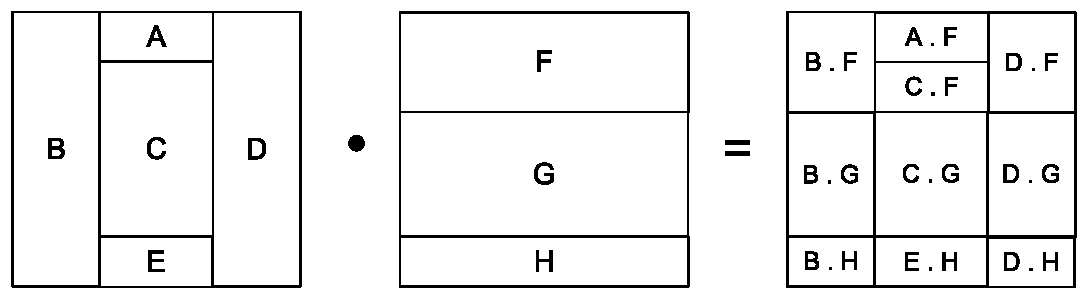
\includegraphics[scale=0.35]{figs/guiding-zipwith-partitions}
\end{center}
%
The number of partitions in the result depends on the number of partitions in the input arrays, which is a static property, as well as the \emph{sizes} of those partitions, which can be a dynamic property.

Repa~3 includes the original @zipWith@ as well as our new @szipWith@ function. With plain @zipWith@, if the overall shape of the source arrays is different, then the shape of the result is their intersection. Performing this intersection is straightforward when there is no internal structure to worry about. In contrast, @szipWith@  preserves the structure of the second source array, but the overall shape of both source arrays must match. 



% -----------------------------------------------------------------------------
\subsection{Cursored Arrays}
\label{section:Cursored}

\begin{figure}
\begin{small}
\begin{code}
data C   -- The type index for cursored arrays.

instance Source C sh a where
  data Array C sh e
     = forall cursor. ACursored
     { cursoredExtent :: sh 
     , makeCursor     :: sh -> cursor
     , shiftCursor    :: sh -> cursor -> cursor
     , loadCursor     :: cursor -> e }
  extent (ACursored ex _     _ _)     = ex
  index  (ACursored _  makec _ loadc) = loadc . makec
  linearIndex (ACursored sh makec _ loadc)
         = loadc . makec . fromIndex sh

instance Load C DIM2 e where
 loadP (ACursored (DIM2 w h) makec shiftc loadc) marr
  = fillCursoredBlock2P ...
        
type PD5 = P C (P D (P D (P D (P D X))))
mapStencil2 :: Source r sh a 
  => Boundary a     -> Stencil DIM2 a
  -> Array r DIM2 a -> Array PD5 DIM2 a
\end{code}
\end{small}
\caption{Cursored Arrays}
\label{figure:Cursored}
\end{figure}

The cursored arrays of \cite{Lippmeier:Stencil} are used to optimise stencil convolutions, by sharing intermediate values between the computation of adjacent pixels. Figure~\ref{figure:Cursored} contains the definition of cursored arrays using our new type-indexed framework. The @Array@ declaration in Figure~\ref{figure:Cursored} takes the role of the @Generator@ from Repa~2, with the role of @makeCursor@, @shiftCursor@ and so on being as per \cite{Lippmeier:Stencil}. 

The definition of @fillCursoredBlock2P@ in the @Load@ instance of Figure~\ref{figure:Cursored} is as per \cite{Lippmeier:Stencil}. As discussed there, its definition contains loops that have been hand-specialised with the unroll-and-jam transformation  \cite{Carr:unroll-and-jam} to separate array reads from array writes. This in turn enables LLVM's global value numbering transformation \cite{Rosen:global-value-nubering}, which recovers sharing of intermediate results between the computation of successive array elements. To improve cache performance, these loops also traverse the source and result arrays in column-wise order, as per the diagram in \S\ref{section:Interleaved}. This means that @fillCursoredBlock2P@ is specialised for arrays of rank-2, hence the @DIM2@ constraint in the @Load@ instance it is used in. 

The @mapStencil2@ function takes a stencil definition, a source array, a description of what to do at the boundary; and produces a partitioned array. This function is also specialised to rank-2 arrays, so the result is split into five partitions, one for inner region and one for each of the four borders. As the use of cursored arrays tends to increase the size of the intermediate code due to loop unrolling, we used a Cursored (@C@) array for the inner region only, defining the borders in terms of Delayed (@D@) arrays. The runtime cost of computing the border regions is typically only a tiny fraction of the cost of computing the internal region, and using delayed arrays for the borders keeps the compile-times and resulting executable size down.


\clearpage{}
\section{Applications and Pragmatics}
\label{sec:performance}

In this section we discuss two end-user applications that were first written with Repa 2, and then modified to work with Repa 3 by the first author. Providing a better way to implement these applications was the reason we started this paper. The first is available in the @gloss-examples@ package, and the second in the @repa-examples@ package. Gloss is a graphics library that depends on Repa.


% -----------------------------------------------------------------------------
\subsection{Fluid Flow}
\label{section:FluidFlow}

Figure~\ref{figure:Fluid} shows output from a fluid flow solver written by Ben \mbox{Lambert-Smith}. This is an implementation of Jos Stam's stable fluid algorithm \cite{Stam:StableFluids}, which is a fast approximate algorithm intended for animation and games, rather than accurate engineering simulation. It performs a finite time-step simulation on a 2-d grid. It is numerically stable for arbitrary sized time-steps, which makes it attractive for real-time animation where the frame-rate of the simulation may vary depending on system load. We discuss the difference between the three images of Figure~\ref{figure:Fluid} in \S\ref{section:Relaxation}.

The fluid is represented as a pair of 2-d arrays, one for the density at each point, and one for the velocity. The density is a scalar floating point value, while the velocity is a 2-d vector. The majority of the runtime is spent in a function called \emph{the linear solver}, which performs matrix relaxation involving the discrete Laplace operator ($\nabla^2$). The linear solver is used to diffuse the density and velocity fields throughout the grid, as well as apply a projection operator to the velocity field, which makes it mass-preserving \cite{Stam:StableFluids}.

Our implementation of the linear solver uses Repa's support for stencil convolution, using the cursored arrays from \S\ref{section:Cursored}, and repeatedly computes the following for each grid element:
$$
u''_{i,j} = (u_{i,j} + a ~.~ (u'_{i-1,j} ~+~ u'_{i+1,j} ~+~ u'_{i,j-1} ~+~ u'_{i,j+1})) ~/~ c
$$
For each time step we perform several relaxation iterations to allow the solution to converge. In the above equation, $u$ is the grid in the previous time step, $u'$ is the grid in the current time step and the previous relaxation iteration, and $u''$ is the grid in the current time step and current iteration. The $a$ and $c$ values are constants determined by simulation parameters, such as the diffusion rate.

The linear solver is written to be polymorphic in the type of array elements. It is then specialised to 2-d vectors (for the velocity) as well as scalar floats (for the density) using GHC's specialisation pragmas \cite{PeytonJones:RewriteRules}. 


% ----------------------------------------------------------------------------
\begin{figure}
\begin{center}
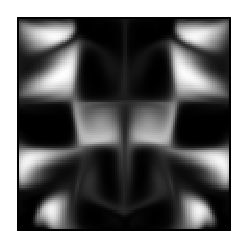
\includegraphics[scale=0.75]{figs/fluid/0100-jacobi4}

\includegraphics[scale=0.75]{figs/fluid/0100-jacobi10}

\includegraphics[scale=0.75]{figs/fluid/0100-jacobi100}
\caption{Fluid Solver output for 4, 10, and 100 Jacobi iterations.}
\label{figure:Fluid}
\end{center}
\end{figure}


% ----------------------------------------------------------------------------
\subsubsection{Scheduling and Smallness Hints}
\label{section:Smallness}
In the Repa version, the linear solver is called four times: once on the scalar density field, and three times on the vector velocity field. Each time it is called, it iteratively performs 40 convolutions with the appropriate stencil, for a total of 160 convolutions per time-step. As the algorithm is intended for real-time simulation, at 30 frames (steps) per second it must perform $30 \times 160 = 4800$ convolutions per second, or one every 200 microseconds. This interval is of the same order of magnitude as the context switch latency on a typical desktop operating system \cite{Li:ContextSwitch}.

When benchmarking the fluid solver using ThreadScope~\cite{Jones:ThreadScope}, we noticed that for a grid of size $100 \times 100$ it was spending over half its time stalled while waiting for worker threads to be scheduled. For context, with a single thread, a grid of size $150 \times 150$ is about largest that will run smoothly at 30 frames per second on our desktop machine. We present concrete numbers in Figure~\ref{figure:FluidRuntime}.

\begin{figure}
\begin{center}
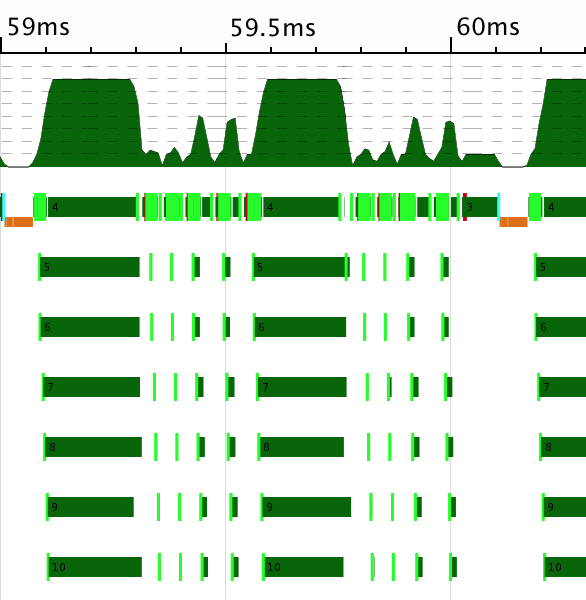
\includegraphics[scale=0.2]{data/fluid/par}
\hspace{2em}
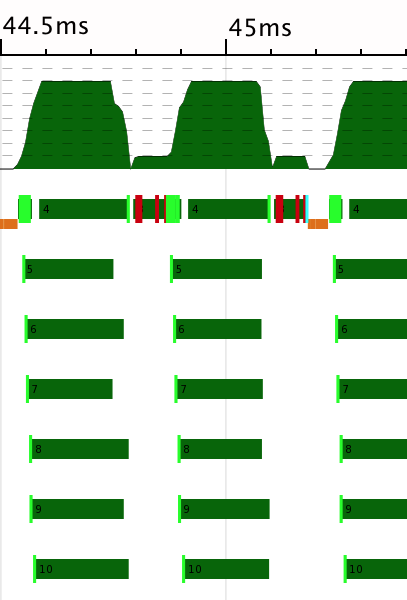
\includegraphics[scale=0.2]{data/fluid/seq}
\end{center}
\caption{Fluid Thread Activity}
\label{figure:FluidActivity}
\end{figure}

% -----------------------------------------------
\begin{figure}
\begin{small}
\begin{code}
data S r
instance Source (S r) sh e
 data Array (S r) sh e 
        = HintSmall (Array r sh e)
 ...

instance ( Shape sh, Load r sh e) 
        => Load (S r) sh e where
 loadP (HintSmall arr) marr = loadS arr marr
 loadS (HintSmall arr) marr = loadS arr marr

type PS5 = P C (P (S D) (P (S D) (P (S D) (P (S D) X))))
mapStencil2 :: Source r DIM2 a 
  => Boundary a     -> Stencil DIM2 a
  -> Array r DIM2 a -> Array PS5 DIM2 a
\end{code}
\end{small}
\caption{Smallness Hints}
\label{figure:SmallnessHints}
\end{figure}


The left of Figure~\ref{figure:FluidActivity} is a ThreadScope plot for the $100 \times 100$ version showing the problem. This plot was taken on an $2\times$QuadCore Intel Harpertown server running Linux Kernel 2.6.32. To minimise the chance of our benchmark being interrupted by the operating system, it was run with only 7 threads (out of 8 possible), leaving the final core for the OS. We use thread affinity to bind each Haskell thread to a single core. In the figure, the 7 horizontal traces show the period each thread was active. The graph at the top shows how many threads were active at each point in time. 

The graph shows two bursts of high activity where the benchmark was performing a matrix relaxation step, and the start of a third one on the far right hand side. As mentioned in \S\ref{section:FluidFlow}, the matrix relaxation is performed using a stencil convolution, which uses the partitioned array representation from \S\ref{section:Partitioned}. Each burst of high activity, where the plot shows all seven threads active, corresponds to the computation of the \emph{inner} region of the array. The four short bursts after it correspond to the computation of the border regions. Because computation of a border region is so little work, more time is spent waiting for the computation to be scheduled than actually computing it.

We address this problem with \emph{smallness hints}, which are wrappers for Repa's usual Delayed (@D@) and Cursored (@C@) type indices. The definition is given in Figure~\ref{figure:SmallnessHints}. Whereas the application of @computeP@ from \S\ref{section:Partitioned} to an array of type @Array D DIM2 Int@ will proceed in parallel, application to an @Array (S D) DIM2 Int@ will proceed sequentially. This behaviour is straightforward to add to our existing framework, as the evaluation method for each array representation is given by the corresponding instance of the @Load@ class. Given some inner representation @r@, the @Load@ instance for @S r@ simply redirects applications of both @loadP@ and @loadS@ to the @loadS@ method for @r@. 

We force the borders of a partitioned array to be evaluated sequentially by modifying the definition of @mapStencil2@ from \S\ref{section:Partitioned}. All that is needed is to wrap the existing border definition in the @HintSmall@ constructor. The effect on the type of @mapStencil2@ is also shown in Figure~\ref{figure:SmallnessHints}.

The ThreadScope plot in the right of Figure~\ref{figure:FluidActivity} is for the same benchmark, now using smallness hints for the border partitions. Now only the main thread is active between each high-activity burst, yet the period of low activity is shorter. 

There is a design choice about whether to preserve smallness hints in the result of an @smap@ operation \S\ref{section:Structured}. Although computation of a particular region in a delayed array may correspond to a small amount of work, after we map a function across every element, computation of the same region in the result may be more expensive. For now we arrange @smap@ to preserve the smallness hint in the result array, though we will return to this in \S\ref{section:HintInteraction}.


% ----------------------------------------------------------------------------
\subsubsection{Gauss-Seidel vs Jacobi relaxation}
\label{section:Relaxation}
The reference C implementation of Jos Stam's fluid flow algorithm was supplied with \cite{Stam:StableFluids}. The linear solver in this version uses Gauss-Seidel matrix relaxation while we use Jacobi relaxation. Relative to the equation in \S\ref{section:FluidFlow}, Gauss-Seidel relaxation replaces the $u'_{i-1,j}$ and $u'_{i,j-1}$ terms with $u''_{i-1,j}$ and $u''_{i,j-1}$ respectively. In the reference version these array elements are read from the array currently being written to. Jacobi relaxation uses the equation as written. 

Although the ``fast forwarding'' of array elements in Gauss-Seidel reduces the number of iterations needed to achieve convergence, its use of destructive update makes it difficult to parallelise. Destructive update also causes problems for optimising compilers such as LLVM (which GHC uses for back-end compilation) as they must worry about potential aliasing between the source and result arrays. In contrast, Jacobi relaxation is kinder to optimising compilers, and easier to parallelise, but requires more iterations than Gauss-Seidel as it does not converge as fast.

For Stam's algorithm, the penalty for using an insufficient number of iterations is an unattractive image with too much numerical dissipation \cite{Stam:StableFluids}. Figure~\ref{figure:Fluid} shows the result of simulating 100 time steps from identical initial conditions, using 4, 10 and 100 Jacobi iterations in the linear solver. For low iteration counts, the swirls present in the right-most image do not appear in the output.

To ensure a fair comparison, our Repa implementation using Jacobi relaxation must use more iterations than the reference implementation. We determined an appropriate number by first simulating the initial conditions used in Figure~\ref{figure:Fluid} using 1000 Gauss-Seidel iterations, treating this as the ideal output. We then measured the mean-square error between the ideal output, and the output using 20 Gauss-Seidel iterations, which is what Stam's reference implementation uses. Finally, we increased the number of Jacobi iterations until the error in the output was reduced to the same level as the reference version. Using 38 Jacobi iterations achieves the same error figure, which we round up to 40 for good measure.



% -----------------------------------------------------------------------------
\subsubsection{Comparison}
Figure~\ref{figure:FluidRuntime} shows the relative runtimes between Stam's C implementation using Gauss-Seidel relaxation (with 20 iterations), and the same program modified to use Jacobi relaxation (with 40 iterations). We also show relative runtime for the Repa version using Jacobi relaxation with 1, 2 and 4 threads. 

The overall shape of this plot is as we would expect. At small array sizes the sequential C versions are faster as they preallocate buffers for the source and result arrays, and swap them after every iteration. This improves data locality, reducing the cache miss rate. In contrast, the Repa version allocates a fresh result buffer for every iteration, leaving old buffers to be reclaimed by the garbage collector. 

At large array sizes, the working set no longer fits in cache and the single threaded Repa Jacobi solver is faster than the C version. This is because cursored arrays allows the Repa version to share intermediate computations, which reduces overall instruction count and memory bandwidth. For large array sizes the benchmark is memory bound, so performance does not scale linearly with an increased number of threads. 

The C reference implementation could be improved by hand-applying the unroll-and-jam transformation that is baked into the Repa library. We tried various permutations of @-funroll-loops@ when compiling with GCC 4.2.1, but inspection of the assembly output revealed it was not recovering the same inter-stencil sharing as the Repa version due to aliasing problems --- even though the loops were indeed unrolled. Compiling with Clang 3.0 (which uses LLVM for the backend) did not significantly improve matters. On the other hand, we could also improve the Repa version by preallocating the source and result arrays and using the @ForeignPtr@ support to swap and reuse the same buffers between iterations.


\begin{figure}
% GNUPLOT: LaTeX picture with Postscript
\begingroup
  \makeatletter
  \providecommand\color[2][]{%
    \GenericError{(gnuplot) \space\space\space\@spaces}{%
      Package color not loaded in conjunction with
      terminal option `colourtext'%
    }{See the gnuplot documentation for explanation.%
    }{Either use 'blacktext' in gnuplot or load the package
      color.sty in LaTeX.}%
    \renewcommand\color[2][]{}%
  }%
  \providecommand\includegraphics[2][]{%
    \GenericError{(gnuplot) \space\space\space\@spaces}{%
      Package graphicx or graphics not loaded%
    }{See the gnuplot documentation for explanation.%
    }{The gnuplot epslatex terminal needs graphicx.sty or graphics.sty.}%
    \renewcommand\includegraphics[2][]{}%
  }%
  \providecommand\rotatebox[2]{#2}%
  \@ifundefined{ifGPcolor}{%
    \newif\ifGPcolor
    \GPcolorfalse
  }{}%
  \@ifundefined{ifGPblacktext}{%
    \newif\ifGPblacktext
    \GPblacktexttrue
  }{}%
  % define a \g@addto@macro without @ in the name:
  \let\gplgaddtomacro\g@addto@macro
  % define empty templates for all commands taking text:
  \gdef\gplbacktext{}%
  \gdef\gplfronttext{}%
  \makeatother
  \ifGPblacktext
    % no textcolor at all
    \def\colorrgb#1{}%
    \def\colorgray#1{}%
  \else
    % gray or color?
    \ifGPcolor
      \def\colorrgb#1{\color[rgb]{#1}}%
      \def\colorgray#1{\color[gray]{#1}}%
      \expandafter\def\csname LTw\endcsname{\color{white}}%
      \expandafter\def\csname LTb\endcsname{\color{black}}%
      \expandafter\def\csname LTa\endcsname{\color{black}}%
      \expandafter\def\csname LT0\endcsname{\color[rgb]{1,0,0}}%
      \expandafter\def\csname LT1\endcsname{\color[rgb]{0,1,0}}%
      \expandafter\def\csname LT2\endcsname{\color[rgb]{0,0,1}}%
      \expandafter\def\csname LT3\endcsname{\color[rgb]{1,0,1}}%
      \expandafter\def\csname LT4\endcsname{\color[rgb]{0,1,1}}%
      \expandafter\def\csname LT5\endcsname{\color[rgb]{1,1,0}}%
      \expandafter\def\csname LT6\endcsname{\color[rgb]{0,0,0}}%
      \expandafter\def\csname LT7\endcsname{\color[rgb]{1,0.3,0}}%
      \expandafter\def\csname LT8\endcsname{\color[rgb]{0.5,0.5,0.5}}%
    \else
      % gray
      \def\colorrgb#1{\color{black}}%
      \def\colorgray#1{\color[gray]{#1}}%
      \expandafter\def\csname LTw\endcsname{\color{white}}%
      \expandafter\def\csname LTb\endcsname{\color{black}}%
      \expandafter\def\csname LTa\endcsname{\color{black}}%
      \expandafter\def\csname LT0\endcsname{\color{black}}%
      \expandafter\def\csname LT1\endcsname{\color{black}}%
      \expandafter\def\csname LT2\endcsname{\color{black}}%
      \expandafter\def\csname LT3\endcsname{\color{black}}%
      \expandafter\def\csname LT4\endcsname{\color{black}}%
      \expandafter\def\csname LT5\endcsname{\color{black}}%
      \expandafter\def\csname LT6\endcsname{\color{black}}%
      \expandafter\def\csname LT7\endcsname{\color{black}}%
      \expandafter\def\csname LT8\endcsname{\color{black}}%
    \fi
  \fi
  \setlength{\unitlength}{0.0500bp}%
  \begin{picture}(5040.00,3310.00)%
    \gplgaddtomacro\gplbacktext{%
      \csname LTb\endcsname%
      \put(472,496){\makebox(0,0)[r]{\strut{} 0}}%
      \put(472,992){\makebox(0,0)[r]{\strut{} 0.5}}%
      \put(472,1489){\makebox(0,0)[r]{\strut{} 1}}%
      \put(472,1985){\makebox(0,0)[r]{\strut{} 1.5}}%
      \put(472,2482){\makebox(0,0)[r]{\strut{} 2}}%
      \put(472,2978){\makebox(0,0)[r]{\strut{} 2.5}}%
      \put(604,276){\makebox(0,0){\strut{}64}}%
      \put(1179,276){\makebox(0,0){\strut{}96}}%
      \put(1587,276){\makebox(0,0){\strut{}128}}%
      \put(2162,276){\makebox(0,0){\strut{}192}}%
      \put(2570,276){\makebox(0,0){\strut{}256}}%
      \put(3144,276){\makebox(0,0){\strut{}384}}%
      \put(3552,276){\makebox(0,0){\strut{}512}}%
      \put(4127,276){\makebox(0,0){\strut{}768}}%
      \put(4535,276){\makebox(0,0){\strut{}1024}}%
      \put(0,1737){\rotatebox{-270}{\makebox(0,0){\strut{}relative runtime}}}%
      \put(2569,50){\makebox(0,0){\strut{}matrix width}}%
      \put(669,1588){\makebox(0,0)[l]{\strut{}C Gauss-Seidel}}%
      \put(669,1141){\makebox(0,0)[l]{\strut{}C Jacobi}}%
      \put(3777,1737){\rotatebox{-10}{\makebox(0,0)[l]{\strut{}Repa -N1}}}%
      \put(3777,1370){\rotatebox{-10}{\makebox(0,0)[l]{\strut{}Repa -N2}}}%
      \put(3777,943){\rotatebox{-10}{\makebox(0,0)[l]{\strut{}Repa -N4}}}%
    }%
    \gplgaddtomacro\gplfronttext{%
    }%
    \gplbacktext
    \put(0,0){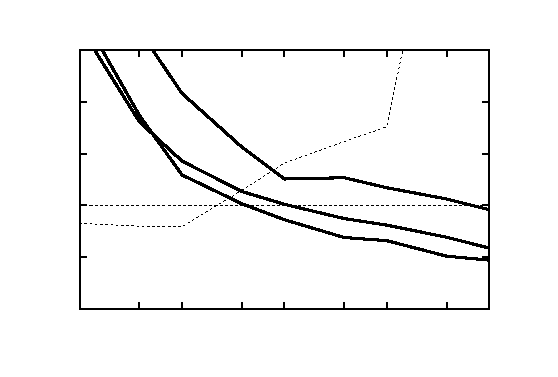
\includegraphics{data/fluid/tesla-size}}%
    \gplfronttext
  \end{picture}%
\endgroup

\caption{Runtimes for Fluid Flow Solver}
\label{figure:FluidRuntime}
\end{figure}


% -----------------------------------------------------------------------------
\subsection{Unbalanced Workloads}
\label{section:Unbalanced}
Figure~\ref{figure:UnbalancedImages} shows three example applications with unbalanced workloads, all written with Repa. The first is a Mandelbrot set visualisation computed with the escape-time algorithm. In the output image, the pixels in the (approximate) Mandelbrot set are rendered black and take about 10 times longer to compute than the others.


% -----------------------------------------------------------------------------
\begin{figure}
\begin{center}
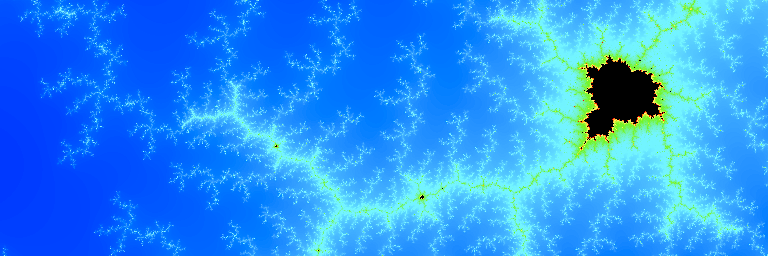
\includegraphics[scale=0.3]{figs/mandel/mandel-lightened}\\
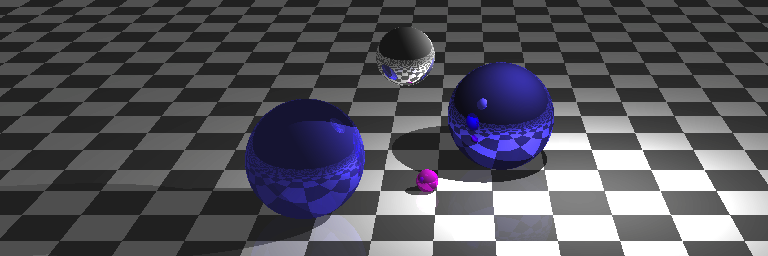
\includegraphics[scale=0.3]{figs/ray/ray-lightened}\\
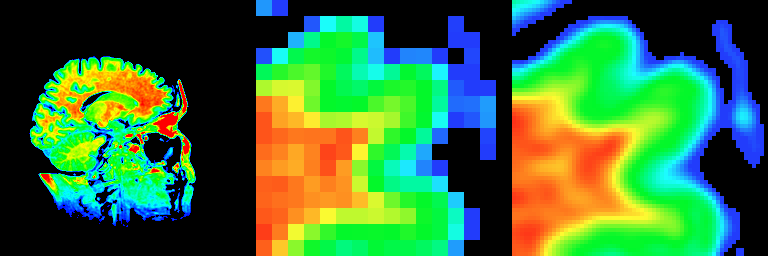
\includegraphics[scale=0.3]{figs/spline/spline-montage}
\caption{Unbalanced Workloads}
\label{figure:UnbalancedImages}
\end{center}
\end{figure}

The second is output from a real-time ray tracer, where parts of the image showing many reflections take longer to compute than the others. Although ray tracing is known in the folklore as ``embarassingly parallel'' as every pixel in the output can be computed independently, it is not embarrassingly \emph{data parallel} due to the unbalanced workload.

The final example is an interpolator for volumetric data, which implements the algorithm described in \cite{Sorokina:Spline}. This example was written by Michael Orlitzky using Repa 2, and then modified to work with Repa 3 by the first author. The left-most image at the bottom of Figure~\ref{figure:UnbalancedImages} shows one slice though a $256 \times 256 \times 109 \times 16$-bit data volume from a Magnetic Resonance Imaging (MRI) machine. The bottom-center image is from the source data, and shows a scaled region of the top-right portion of the brain. The bottom-right image shows the same region after interpolation. In a straightforward implementation, every element in the output volume is computed independently and takes the same amount of time. However, we can improve the overall runtime by returning a constant zero value (black pixel) for voxels corresponding to the air surrounding the physical object. This is done by summing the surrounding voxels in the source data, and testing the sum against a user defined threshold. This is faster than calculating the true interpolated result, but again makes the workload unbalanced.


% -----------------------------------------------------------------------------
\subsubsection{Spacial Correlation and Interleaved Evaluation}
\label{section:Interleaved}
The workloads of our three examples are unbalanced because the cost to compute each array element is not uniform throughout the array. The standard Repa evaluation method chunks the underlying row-major vector evenly between the available threads. When using cursored arrays we instead proceed column-wise as this is more cache-efficient when performing convolutions on 2-d matrices. The figure below shows both of these methods, assuming we are computing the matrix with three threads.
%
\begin{center}
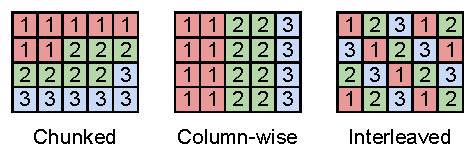
\includegraphics[scale=0.8]{figs/guiding-eval-order}
\end{center}
%
With both the Chunked and Column-wise method, the spacial correlation between features in the result array, and computational workloads maps directly onto the physical processors. The left of Figure~\ref{figure:InterpolatorThreads} is a ThreadScope plot that shows the effect of this correlation in sharp relief. The plot is for the interpolator on seven threads, which shows the threads that compute non-zero data in the result take significantly longer to run. The plot is for the entire run of the program, and the high-activity bursts at the beginning and end are due to reading source data and writing the output to file.

A well known solution to this problem is to move to an interleaved evaluation method instead \cite{Salmon:RayTracer}, also shown in the figure above. When applied to ray tracing this approach is classically known as \emph{image space partitioning} to distinguish it from \emph{object space partitioning} which divides the model being rendered. As with all static load-balancing strategies, there is still a chance that the runtime-workload will correlate with the assigned thread index, though this would be unlikely for the three applications shown in Figure~\ref{figure:UnbalancedImages}. Lee and Raghavendra~\cite{Lee:RayTracerLoadBalancing} compare related strategies. 

\begin{figure}
\begin{center}
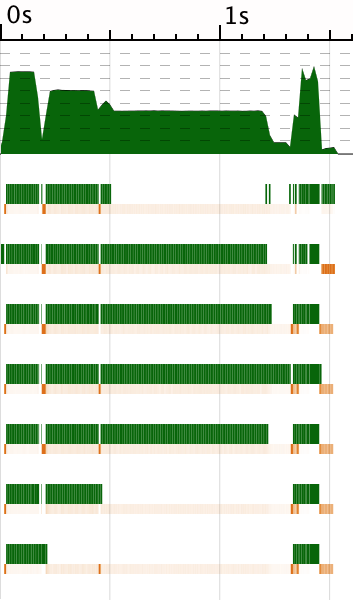
\includegraphics[scale=0.25]{data/spline/spline3-unbalanced}
\hspace{3em}
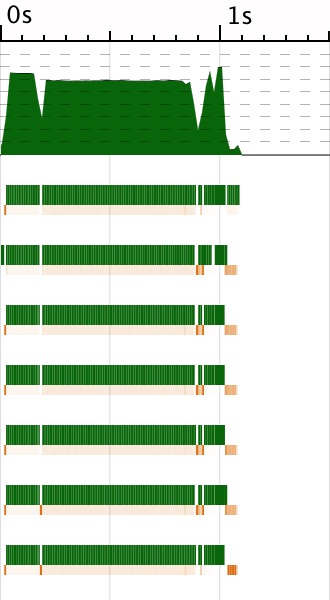
\includegraphics[scale=0.25]{data/spline/spline3-interleave}\\
\caption{Interpolator Thread Activity}
\label{figure:InterpolatorThreads}
\end{center}
\end{figure}

We implement our new interleaved evaluation method similarly to the smallness hints from \S\ref{section:Smallness}, with the main definitions given Figure~\ref{figure:InterleaveHints}. Whereas application of @computeP@ to an array of type @Array D DIM2 Int@ will use chunked evaluation, application to an @Array (I D) DIM2 Int@ now uses interleaved evaluation, implemented by @fillInterleavedP@. The right of Figure~\ref{figure:InterpolatorThreads} shows the result of using interleaved evaluation for the interpolator. All threads now run for approximately the same period of time, and of the overall runtime of the program is shorter. 

% Note that although interleaved evaluation causes different threads to write to alternate elements, this does not in itself cause serious cache contention. The first time one thread tries to write to a cache line owned by another it will be stalled. This allows time for the second thread to advance further, which reduces the likelihood of a subsequent conflict. We verified the lack of cache-contention by integrating the thread activity plots for out three benchmarks over time. The total workload (in units of thread-seconds) is identical for interleaved and non-interleaved evaluation, for each benchmark. 


% -----------------------------------------------------------------------------
\begin{figure}
\begin{small}
\begin{code}
data I r1
instance Source (I r1) sh e
 data Array (I r1) sh e
        = HintInterleave (Array r1 sh e)

instance ( Shape sh, Load D sh e) 
        => Load (I D) sh e where
 loadP (HintInterleave (ADelayed sh getElem)) marr 
   = fillInterleavedP (size sh) (unsafeWriteMArr marr) 
                                (getElem . fromIndex sh) 
 loadS (HintInterleave arr) marr = loadS arr marr

instance Structured rs a => Structured (I rs) a where
 type TR (I rs) = I (TR rs)
 ...
\end{code}
\end{small}
\caption{Interleave Hints}
\label{figure:InterleaveHints}
\end{figure}


% -----------------------------------------------------------------------------
\subsubsection{Hint Propagation and Interaction}
\label{section:HintInteraction}
The @Load@ instance in Figure~\ref{figure:InterleaveHints} only works for Delayed (@D@) arrays, and not Cursored (@C@) arrays as well. As described in \S\ref{section:Cursored}, cursored arrays are used to share intermediate computations between adjacent array elements, and this process depends on a particular traversal order. As adjacent elements must be computed in the same loop iteration, using interleaved evaluation with cursored arrays would be of no benefit.

Smallness hints and interleave hints interact in a natural way. If a delayed array is wrapped in an Interleave (@I@) hint, this signals that its parallel computation will be unbalanced. If it is then wrapped in a Smallness (@S@) hint as well, this signals that it is a small amount of work \emph{relative} to some larger computation. The combination of hints yields a type index of @(S (I D))@. When the array is finally computed, the instances given in Figures \ref{figure:SmallnessHints} and \ref{figure:InterleaveHints} effectively ignore the interleave hint, as the sequential evaluation enforced by smallness cannot itself be unbalanced. If the two hints are applied in the other order, to yield an index of @(I (S D))@ then there is no available @Load@ instance, because hinting that a sequential computation is unbalanced does not make sense.

Finally, note that the @Structured@ instance in Figure~\ref{figure:InterleaveHints} propagates the interleave hint to the result representation. The declaration of @Structured@ was given in Figure~\ref{figure:Structured}. We preserve this hint because the @Structured@ class methods, namely @smap@ and @szipWith@ are bulk operations, meaning they apply the same function to every array element. In practice, it is highly unlikely that applying such an operation to an array defining an unbalanced workload would make it \emph{more} balanced, so it is better to retain the unbalancedness. For example, suppose we apply our ray-tracer to a 3d model and then convert the output image to greyscale:
%
\begin{small}
\begin{code}
  image :: Array U DIM2 Float
  image = computeP $ smap toGreyScale $ raytrace model
\end{code}
\end{small}
%
The result of evaluating @raytrace model@ will have the type \\ @Array (I D) DIM2 (Float, Float, Float)@, where the tuple contains red, green, blue color values. Applying @smap toGreyScale@ the produces @Array (I D) DIM2 Float@, where the result gives a luminance value for each pixel. The array defined by the @raytrace@ is unbalanced, and when fused with @toGreyScale@ it remains unbalanced. 




\section{Challenges of Array Fusion}
This section summaries the remaining challenges we see to the Repa-style approach to array fusion. We continue the similarly named section in \cite{Lippmeier:Stencil}.


% -----------------------------------------------------------------------------
\subsection{Unboxing Outside Loops}

In \cite{Lippmeier:Stencil} we used boilerplate code involving @deepSeqArray@ to force GHC to unbox array objects outside of loops. Adding this code worked around limitations in the simplifier for GHC's core IR. For example, consider the following function which takes an array of indices, a matrix and yields elements from the matrix diagonal:
\par
\begin{small}
\begin{code}
  diagonals :: Array U DIM1 Int -> Array U DIM2 Int
            -> Array U DIM1 Int
  diagonals xs ys
   = computeP $ R.map (\i -> ys `index` (DIM2 i i)) xs
\end{code}
\end{small}
%
As the @ys@ array is only used inside the worker function passed to @map@, with lazy evaluation this array will only be demanded if @xs@ contains at least one element. As the GHC simplifier mostly\footnote{In GHC 7.4.1, non-termination is not preserved by eta expansion, but correct termination behaviour can be gained with @-fpedantic-bottoms@.} tries to preserve the termination behaviour of the program during transformation, it does not float this unboxing out of the loop. It must guard against the case where evaluation of @ys@ diverges, hence the components of @ys@ end up being unboxed repeatedly for every iteration. Even with pointer tagging \cite{Marlow:PointerTagging}, the cost of unboxing values in inner loops can easily dominate the runtime of an array program.

With Repa 2 and GHC 7.2 we needed to use @deepSeqArray@ to place a demand on the components of @ys@, to ensure their unboxings are floated outside the loop:
\par
\begin{small}
\begin{code}
  diagonals xs ys
   = ys `deepSeqArray` 
     computeP $ map (\i -> ys `index` (DIM2 i i)) xs
\end{code}
\end{small}
%
In GHC 7.4.1 we implemented case-floating. This transform operates much like let-floating \cite{PeytonJones:LetFloating}, except that it moves single-alternative case expressions. 

\eject
With case-floating, instead of needing @deepSeqArray@ we can achieve fast code by using a lighter-weight bang pattern:
\par
\begin{small}
\begin{code}
  diagonals xs !ys = ...
\end{code}
\end{small}
%
This then desugars to:
%
\begin{small}
\begin{code}
  diagonals xs ys
   = case ys of { _ -> 
     computeP $ map (\i -> ys `index` (DIM2 i i)) xs }
\end{code}
\end{small}
%
When the definition of @index@ is inlined we get:
%
\begin{small}
\begin{code}
  diagonals xs ys
   = case ys of  { _ -> 
     computeP $ map (\i -> 
      case ys of { AUnboxed sh uvec -> 
      case sh of { DIM2 w h -> ..w h uvec i..}}) xs }  
\end{code}
\end{small}
%
Now, as @ys@ is demanded on entry to the function, the inner match against @AUnboxed sh uvec@ can be unconditionally moved to top level. However, hoisting the match against @DIM2 w h@ is only sound when the shape of an array is defined as a strict field, though from Figure~\ref{figure:Source} we see that it is. Moving the match on @DIM2 w h@ to the outer case expression based on this strictness information is our new case-floating transform: 
%
\begin{small}
\begin{code}
  diagonals xs ys
   = case ys of { AUnboxed sh uvec ->
     case sh of { DIM2 w h         -> 
      computeP $ map (\i -> ..w h uvec i..) xs }}
\end{code}
\end{small}
%
In practice, we advise users to add bang patterns to \emph{all} array parameters for functions using the Repa library. Although the @xs@ parameter above does not need one, adding it does not hurt, and this is an easy-to-follow rule. 

Sadly, bang patterns are not always sufficient. Suppose @ys@ is defined as a top-level CAF:
\par
\begin{small}
\begin{code}
  ys = fromList ...
  diagonals xs
   = computeP $ map (\i -> ys `index` (DIM2 i i)) xs
\end{code}
\end{small}
%
In this situation the language definition does not allow us to place a bang on @ys@. This would imply that @ys@ should be evaluated as soon as the program starts, which is problematic if it happened not to terminate. Instead we add a @seq@, like so:
\par
\begin{small}
\begin{code}
  ys = fromList ...
  diagonals xs = ys `seq` 
     computeP $ map (\i -> ys `index` (DIM2 i i)) xs
\end{code}
\end{small}
%
The @seq@ desugars to a case-expression as above. The fact that @seq@s must still be added to get efficient code is not kind to beginning Haskell programmers, but we do not see a way to avoid it with the current language semantics. 


% -----------------------------------------------------------------------------
\subsection{Fake Nested Parallelism via Laziness}
The following example is like @diagonals@ from the previous subsection, except that it first increments every element in the matrix.
\par
\begin{small}
\begin{code}
 diagonals2 :: Array U DIM1 Int -> Array U DIM2 Int
            -> Array U DIM1 Int
 diagonals2 xs ys
  = let ys2 :: Array U DIM2 Int
        ys2 = computeP $ map (+ 1) ys
    in  computeP $ map (\i -> ys2 `index` (DIM2 i i)) xs
\end{code}
\end{small}
%
At runtime, the binding for @ys2@ involving the first @computeP@ will be suspended by lazy evaluation. This binding will be forced by the second @computeP@ expression when it tries to evaluate the initial element in the overall result of @diagonals2@. When one parallel computation invokes another it is nested parallelism, which Repa does not support. Our current implementation will print a warning to @stderr@ and then run the inner @computeP@ sequentially. 
%
Although this behaviour provides the expected result at the value level, sequential evaluation is unlikely to be what the user intended --- especially because they wrote @computeP@ (with a parallel @P@). To ensure that both applications of @computeP@ actually run in parallel, evaluation of @ys2@ must complete before the second @computeP@ starts. Once again, this can be fixed with a bang pattern:
%
\begin{small}
\begin{code}       
 diagonals2 xs ys
  = let ys2 :: Array U DIM2 Int
        !ys2 = computeP $ map (+ 1) ys
    in  computeP $ map (\i -> ys2 `index` (DIM2 i i)) xs
\end{code}
\end{small}
%
The Repa library is written so that when the first parallel computation is evaluated, it unsafely initialises a globally shared gang of threads (with @unsafePerformIO@). All subsequent parallel computations run on this single gang of threads, and hence only one can run at a time. We do \emph{not} create thread gangs dynamically because a single, well balanced data parallel computation is always enough to keep all threads busy. If we had multiple gangs running concurrently, then they would contend for cache and thrash the OS scheduler. Importantly, using an unsafely initialised gang of threads does \emph{not} violate observational purity (other than on @stderr@), because all Repa computations still return the correct value, even though nested computations may run sequentially.

Should we change Repa to support slow nested parallel computations that the user probably didn't mean to write? Probably not! Until we have a way to statically guarantee that only one parallel computation runs at a time, we offer the following function in the default API:
\par
\begin{small}
\begin{code}
 computeMP :: (Load  rs sh e, Target rt e, Monad m)
            => Array rs sh e -> m (Array rt sh e)
 computeMP arr
  = let arr2 = computeP arr
    in  arr2 `seq` return arr2
\end{code}
\end{small}
%
The function @computeMP@ is like @computeP@, except that it forces completion at a particular point in a monadic computation. Writing @diagonals2@ with @do@-notation and using @computeMP@ will achieve the same result as adding the bang pattern to @ys2@. In fact, only @computeMP@ is exposed in the top-level Repa module. The user needs to go looking to find @computeP@, before they can get themselves in trouble with fake nested parallelism.

Note that @computeMP@ is parametric in the monad as we only need a well defined notion of sequence, rather than a particular monadic effect. Of course, the user could instantiate this to the @ST@ monad and still run two parallel computations concurrently, just like they could instantiate it to @IO@ and use @forkIO@ to achieve the same result. Both of these operations would be considered ``safe'' in the Haskell development culture. It would be nice if our types could enforce \emph{all} the desired performance characteristics, but as of now they are only a guide.



%!TEX root = ../Main.tex
\section{Related Work}

\begin{itemize}
\item Iteratee Enumerator
\item Conduit, we don't have await and yield. Flows are not monad transformers.
\item Pipes
\item Machines support multiple inputs and fanout.
\item Monad par, is event flow network using IVars.
\item Impala.
\item Hive.
\item Spark.
\item Google Tensorflow
\item Lustre, Lucid sync data flow, Kahn networks.
\item StreamIt, Brook.
\item Scala streams library.
\item FRP libraries, eg reflex.
\end{itemize}


% Repa flow fills a sweet spot between the roles functional array library and analytic database. In terms of the programming model, a key feature of Repa Flow compared with Scoobi and Scalding is that the API carefully distinguishes between operators that run in constant space and those which do not. Systems based on map-reduce make implicit use of a \emph{shuffle} operator that distributes data between the compute nodes. The \emph{shuffle} operator sends data between the nodes in a data-dependent way, which can result in a skewed workload where most data is sent to a subset of nodes while the others are starved. When all source-level queries are converted into map-reduce jobs then there is no systematic way in which skew can be avoided. Taking inspiration from the work on synchronous data flow and Khan networks, we have arranged our API so that most operators execute without buffering. With Repa Flow it is easy to write programs where both buffering and data skew are avoided by construction, or admitted only in a controlled way.


\eject
% -----------------------------------------------------------------------------
\paragraph{Acknowledgements}
Thanks to Ben Lambert-Smith for the original Fluid Flow example, Michael Orlitzky for the interpolation example, and Andres L\"{o}h for discussion about the role of @computeMP@. During the development of Repa 1, Roman Leshchinskiy argued that we should distinguish between array representations at the type level --- he was right. This work was supported in part by the Australian Research Council under grant number LP0989507. 

\bibliographystyle{abbrvnat}
\bibliography{Main}

\clearpage{}
\end{document}

